\section{Post-processing} \label{section:post}
We observed recurring visual artefacts like disconnected road fragments, see Fig. \ref{fig:example} c), in our predicted results. Initially we attempted to resolve this using classical methods such as morphological operations (e.g. erosion, dilation) and median filtering. While these structure based approaches helped by connecting disjoint road segments, they introduced new artefacts in some predictions by merging adjacent roads. Due to the diversity of the images, the exact filter type, shape and size, which worked best for a prediction was sensitive to the road structure. Instead of a manual grid search for the best possible parameters per image, we developed two novel learning based post processing methods.

\begin{figure}
\centering
%   \begin{subfigure}[b]{0.3\linewidth}
%     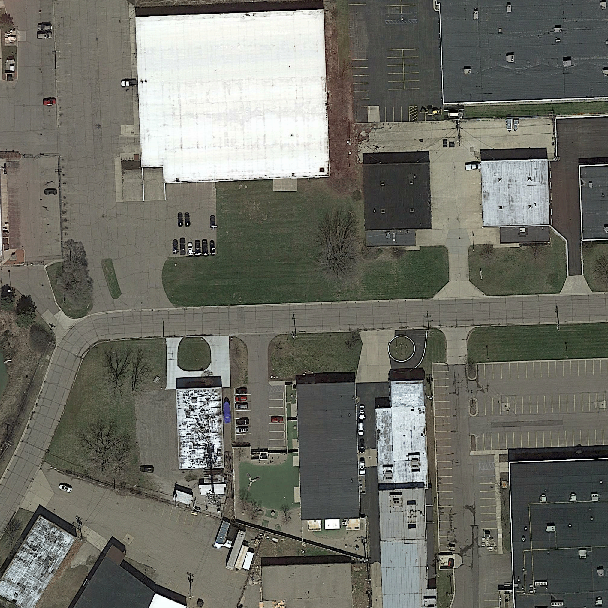
\includegraphics[width=\linewidth]{images/test_105.png}\caption{}
%   \end{subfigure}
  %
  \begin{subfigure}[b]{0.3\linewidth}
    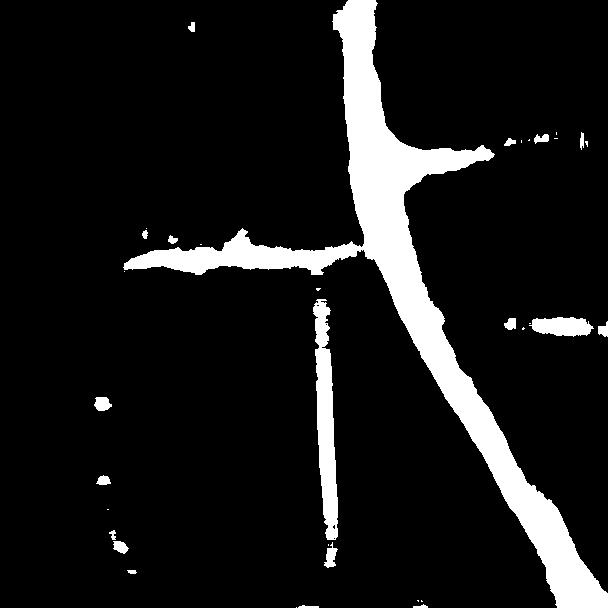
\includegraphics[width=\linewidth]{images/pred_190_orig.png}
    \caption{}
  \end{subfigure}
  %
  \begin{subfigure}[b]{0.3\linewidth}
    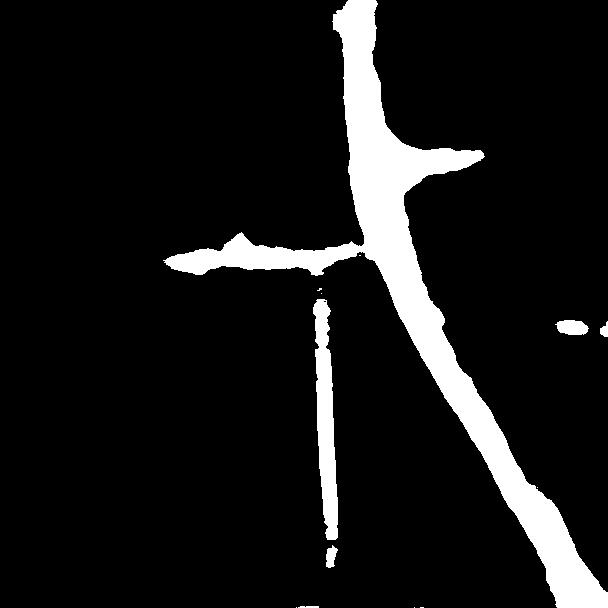
\includegraphics[width=\linewidth]{images/pred_190_simpleunet.jpg}
    \caption{}
  \end{subfigure}
     \begin{subfigure}[b]{0.3\linewidth}
     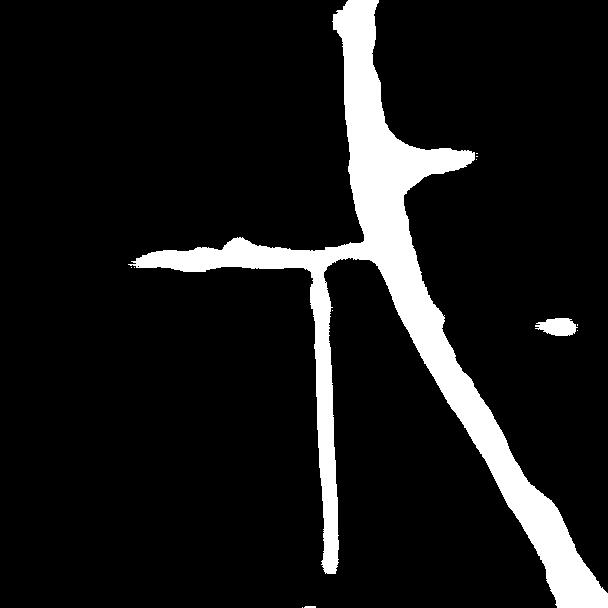
\includegraphics[width=\linewidth]{images/pred_190_pconv_dil3.jpg}
     \caption{}
   \end{subfigure}
  
%   \par\smallskip
%   \begin{subfigure}[b]{0.3\linewidth}
%      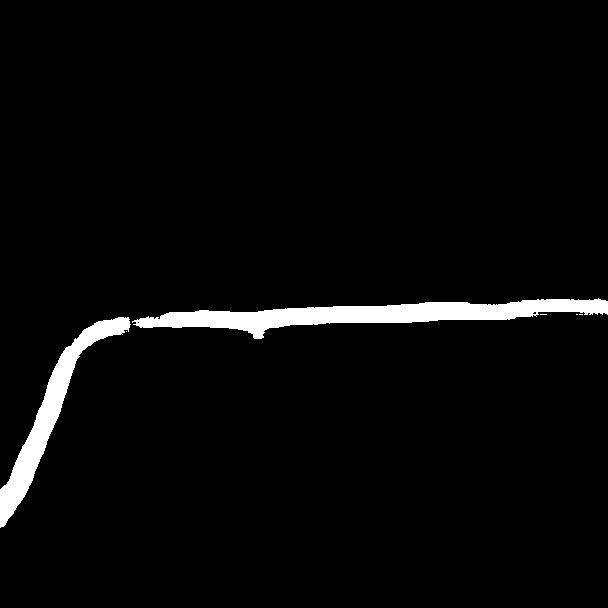
\includegraphics[width=\linewidth]{images/dil_5_pred_105.jpg}\caption{}
%   \end{subfigure}

%   \begin{subfigure}[b]{0.3\linewidth}
%      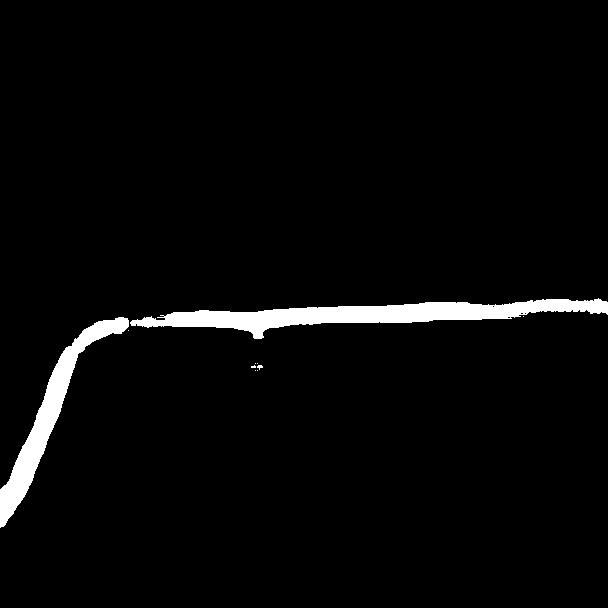
\includegraphics[width=\linewidth]{images/dil_7_pred_105.jpg}\caption{}
%   \end{subfigure}
  \caption{Retrain on binary predictions: 
  a) Original prediction, b) Retrain simple \acrshort{unet},
  c) Retrain \acrshort{unet} with partial convolution and dilation 3.
  }
  \label{fig:postprocessing}
  \vspace{-7mm}
\end{figure}


\subsection{Retraining on binary predicted images} \label{subsec:binary_retraining}
We used the best predictions of the U-Net \& \acrshort{gcdcnn} as a training set and retrained the network to learn how to connect roads by joining lines and to remove noisy predictions.

\subsubsection{Partial convolution} 
Partial convolution layers are commonly used for image inpainting of irregular holes \cite{partialconv}. Instead of learning different morphological filters, we decided to use these layers to inpaint pixels to recreate road images.
%Partial convolutions normalize the output to adjust for a fraction of the missing data. 
When retraining on the binary images, we replaced the normal convolution layers with partial convolution layers as in \cite{partialconv}. 
As seen in Figure \ref{fig:postprocessing} c) this leads to cleaner boundaries between roads and denoised predictions.

\subsubsection{Increasing the receptive field} As seen in Fig. \ref{fig:postprocessing} b), some of the roads still remained disconnected. Increasing the dilation helped to increase the receptive field of the network to learn whether disjoint segments separated by a large black margin indeed constitute a road. This improved the quality of predicted images both for the \acrshort{unet} with partial convolution and the normal \acrshort{unet} as shown in Tables \ref{tab:postprocessingunet} and \ref{tab:postprocessinggcdcnn} in the Appendix. Retraining helped to produce cleaner images, but improved the public score by only 0.199 percentage points due to the 16x16 patch abstraction.

\subsection{Learning with Hough Transformations}
 Another idea we came up with was to nudge the network towards predicting connected roads by explicitly presenting possible connected line fragments. A classical computer vision technique to detect shapes such as lines in images is the so-called Hough transformation \cite{hough}. By looking at the predicted mask and counting the number of pixels that lie on straight lines in specific angles, this method returns all possible lines that exceed a certain threshold. We draw these lines with the width of an average street on the predicted masks, concatenate this image with the prediction and the original RGB image and train a post-processing network (U-Net) on it. Thus, our model is trained on images with 5 channels (RGB, prediction, lines). The network should decide which of these roads (if any) it should keep. 

 This can be interpreted in several different ways. First, one could see it as letting the network learn how to remove predicted roads, thereby concentrating exactly on the parts between already identified road fragments. Secondly, one could also interpret this as a kind of topological prior. The prior probability of another road pixel on the connecting line between two fragments is higher than in any other part of the image. Thirdly, by providing these lines, we give the network an additional set of features, which can be used to improve the current predictions – or can be ignored.

\begin{figure}[h!]
\centering
  \begin{subfigure}[b]{0.22\linewidth}
    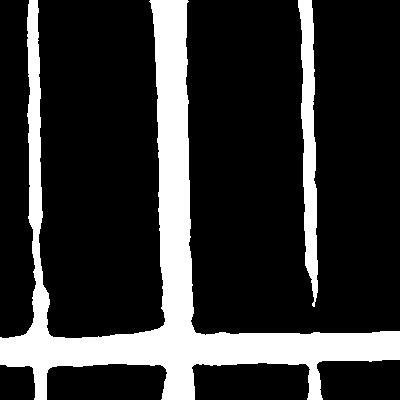
\includegraphics[width=\linewidth]{images/satImage_024_prediction.png}\caption{}
  \end{subfigure}
  %
  \begin{subfigure}[b]{0.22\linewidth}
    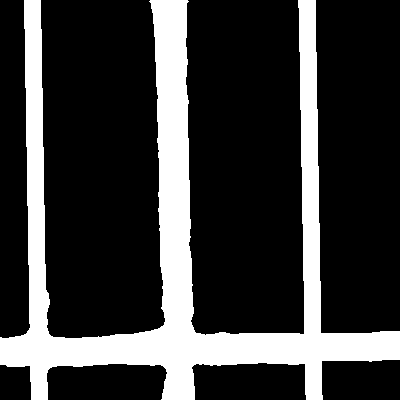
\includegraphics[width=\linewidth]{images/satImage_024_lines.png}\caption{}
  \end{subfigure}
%
   \begin{subfigure}[b]{0.22\linewidth}
    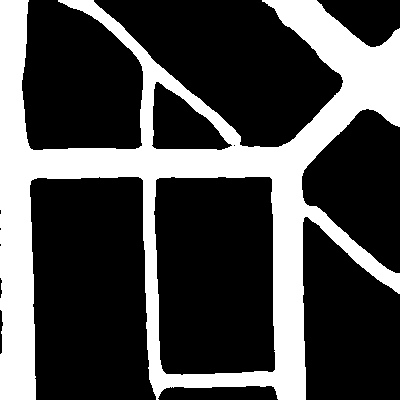
\includegraphics[width=\linewidth]{images/satImage_075.png}\caption{}
  \end{subfigure}
  %
  \begin{subfigure}[b]{0.22\linewidth}
    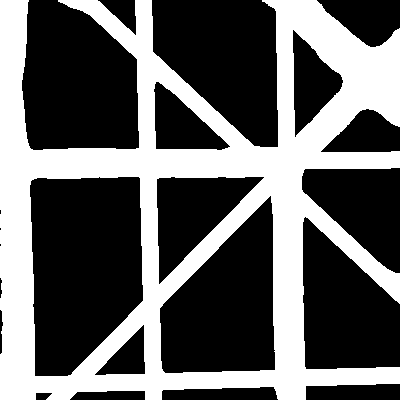
\includegraphics[width=\linewidth]{images/satImage_075-lines.png}\caption{}
  \end{subfigure}
    \caption{Hough Transformations: (a), (c) show the original predictions. (b), (d) show the completed lines.
  %A U-Net is trained on these three images (5-channels) to decide whether to keep the completed lines.
  }
  \label{fig:hough}
\end{figure}

For an illustration of the Hough Transformation, see Fig. \ref{fig:hough}. In the first image (a, b), we see that the lines are very simple and therefore this approach works fine. However, when the road network is more complicated as in (c), there are many wrong lines (d). This leads our model to use the original prediction and mostly ignore the lines. Therefore, this post-processing technique does not help in improving prediction accuracy.

% Further work could be done by including the Hough Transformation lines in the training of the main network in form of a prior, starting in a certain epoch.

\subsection{Ensemble Methods}

Averaging the predictions from different models is another form of post-processing, as it helps to remove artefacts, such as separated road predictions. If at least 50\% of the models predicted a pixel as road, then the ensemble prediction considers it to be road. Afterwards, the predictions are patched as usual. This procedure has shown to significantly improve prediction accuracy, as shown in Section \ref{section:results}.
